\documentclass[10pt,a4paper]{article}
\usepackage[spanish,es-nodecimaldot]{babel}
\usepackage[margin=20mm]{geometry}
\usepackage{microtype,amsmath,graphicx,booktabs,longtable,tabularx,array,xcolor,float,fancyhdr,enumitem,pdfpages}
\usepackage[colorlinks=true,linkcolor=black,urlcolor=blue!55!black]{hyperref}
\graphicspath{{../../img/}{../protoboard/}}
% Identidad: Manual resumido de marca CUC, edición publicada en agosto de 2024.
% Logo vectorial oficial, sin reconstrucción ni modificación de sus elementos.
\usepackage{fontspec}
\usepackage{unicode-math}
\setmathfont{Latin Modern Math}
\defaultfontfeatures{Ligatures=TeX}
\setmainfont{RedHatDisplay}[Path=fuentes/,Extension=.ttf,UprightFont=*-Regular,BoldFont=*-Bold,ItalicFont=*-Italic]
\setsansfont{RedHatDisplay}[Path=fuentes/,Extension=.ttf,UprightFont=*-Regular,BoldFont=*-Bold,ItalicFont=*-Italic]
\definecolor{cucrojo}{HTML}{A3161A}
\definecolor{cucoro}{HTML}{C9A227}
\definecolor{cucgris}{HTML}{595959}
\definecolor{cucplata}{HTML}{CCCCCC}
\newcommand{\logocuc}[1]{
\includegraphics[width=#1]{marca/cuc-logo-vector.pdf}}

\usepackage{titlesec}
\titleformat{\section}{\Large\bfseries\color{cucrojo}}{\thesection.}{.6em}{}
\titleformat{\subsection}{\large\bfseries}{\thesubsection.}{.6em}{}
\hypersetup{linkcolor=cucrojo,urlcolor=cucrojo,pdftitle={Ecualizador: guía de montaje en protoboard},pdfauthor={Leo Rojas, David Orozco, Manuel Castilla}}
\setlength{\headheight}{29pt}
\setlength{\parindent}{0pt}\setlength{\parskip}{5pt}
\setlist{nosep,leftmargin=*}
\pagestyle{fancy}\fancyhf{}\fancyhead[L]{\logocuc{30mm}}\fancyhead[R]{\small Electrónica II · Guía de prototipo}\fancyfoot[C]{\thepage}
\newcommand{\red}[1]{\texttt{\detokenize{#1}}}
\newcommand{\etapa}[3][48mm]{\begin{figure}[H]\centering\includegraphics[width=.98\linewidth,height=#1,keepaspectratio]{circuitos/#2.pdf}\caption{#3}\end{figure}}
\begin{document}
\begin{center}
{\LARGE\bfseries Ecualizador de audio de tres bandas}\par
{\Large Montaje y pruebas en protoboard}\par
\vspace{4mm}
Leo Rojas · David Orozco · Manuel Castilla\\
Universidad de la Costa · Electrónica II\\23 de octubre de 2026
\end{center}
{\color{cucrojo}\rule{\linewidth}{1pt}}

\section{Qué se va a construir}
Un prototipo de la cadena analógica del ecualizador: entrada de línea, preamplificador, filtros de graves, medios y agudos, controles, corrección de fase, sumador y salida de línea. También se montan los detectores de nivel y el filtro para el ADC, de modo que después se pueda conectar el ESP32 sin cambiar esa cadena.

\textbf{Para comenzar:} dos protoboards de 830 puntos, cuatro MCP6004 en DIP-14, 29 resistencias, 23 capacitores, cuatro potenciómetros, tres diodos y dos conectores de audio. La lista detallada aparece en la sección siguiente. Para comprobar el filtrado bastan una fuente regulada de 3,3 V, un generador y un osciloscopio. Para escucharlo, conectar la salida a un parlante activo o a un amplificador externo.

\textbf{Ampliación:} ESP32-DevKitC de 38 pines, pantalla Waveshare de 1,9 pulgadas y tira NeoPixel. El PAM8403 y el parlante interno se describen como una opción aparte; no son necesarios para medir el ecualizador.

Las referencias y las redes de esta guía se obtienen de \red{herramientas/circuito.py}, la misma descripción usada para la PCB D.2. El esquema completo se incluye al final del PDF. Esta guía es un documento independiente de montaje; no reemplaza la versión de PCB de una cara. Las ubicaciones de los integrados son una propuesta de distribución, no evidencia de un montaje físico ya probado.

\section{Materiales para la parte analógica}
\textbf{Compra los MCP6004 en encapsulado DIP-14}, por ejemplo MCP6004-I/P. Los encapsulados SMD requieren adaptador. No reemplazarlos directamente por LM324, TL074 o TL084: el circuito utiliza una sola alimentación de 3,3 V y una referencia cercana a 1,65 V.

En la tabla, las resistencias están expresadas en ohmios y los capacitores en faradios: 10k = 10 k\ensuremath{\Omega}; 100n = 100 nF; 4n7 = 4,7 nF. Usar resistencias de 1/4 W; respetar el 1 \% donde se indica. Para los filtros, capacitores de película con tolerancia de 5 \% o mejor. Los de 100 nF de desacople pueden ser cerámicos.
{\small\begin{longtable}{r p{65mm} p{72mm}}
\toprule Cant. & Componente / valor & Referencias\\\midrule\endhead
1 & 10 & R1\\
1 & 100u 10V & C1\\
5 & 100n & C2, C4, C5, C6, C7\\
9 & 10k 1\% & R2, R3, R8, R9, R10, R13, R14, R25, R26\\
2 & 10u 16V & C8, C19\\
1 & Entrada de línea 3,5 mm & J1\\
2 & 10k & R4, R5\\
1 & 10k log & RV1\\
1 & 1u film & C9\\
1 & 100k & R6\\
1 & 22k 1\% & R7\\
1 & 10 µF bipolar, \ensuremath{\geq} 10 V (ver nota C10) & C10\\
4 & 100n film & C11, C22, C23, C24\\
1 & 47n film & C12\\
5 & 10n film & C13, C14, C15, C17, C18\\
1 & 27k 1\% & R11\\
1 & 56k 1\% & R12\\
2 & 4n7 film & C16, C20\\
1 & 2k7 1\% & R15\\
1 & 5k6 1\% & R16\\
3 & 10 k\ensuremath{\Omega} lineal; rotativo o deslizable con cables & RV2, RV3, RV4\\
5 & 47k 1\% & R17, R18, R19, R20, R21\\
1 & 100k 1\% & R22\\
1 & 100 & R23\\
1 & 47k & R24\\
1 & Salida de línea 3,5 mm & J2\\
1 & 2n2 film & C21\\
3 & 1N4148 & D1, D2, D3\\
3 & 220k & R27, R28, R29\\
4 & MCP6004-I/P, DIP-14 & U1, U2, U3, U4\\
\bottomrule\end{longtable}
}

\textbf{C10:} para esta guía se recomienda 10 µF \emph{bipolar} o no polarizado, con el mismo valor del esquema. Sus dos terminales quedan cerca de VREF en continua; no hay una polarización positiva estable que justifique orientar un electrolítico común. C1, C8 y C19 sí conservan la polaridad indicada en la tabla de conexiones.

\textbf{Potenciómetros:} RV1 es de 10 k\ensuremath{\Omega} logarítmico. RV2, RV3 y RV4 son de 10 k\ensuremath{\Omega} lineal; para la protoboard pueden ser rotativos, aunque el gabinete utiliza deslizables. Identificar el cursor con el multímetro. Los números 1, 2 y 3 de la guía son terminales eléctricos; verificar cómo los enumera el fabricante. El terminal 2 es siempre el cursor.

\subsection{Elementos de montaje e instrumentos}
\begin{tabularx}{\linewidth}{r X}\toprule
Cantidad & Material\\\midrule
2 & Protoboards de 830 puntos para la cadena analógica.\\
1 juego & 100--150 puentes rígidos de 22 AWG y cables cortos; cables macho-hembra para módulos y controles externos.\\
2 & Adaptadores de jack TRS de 3,5 mm a terminales de 2,54 mm, o jacks de panel con cables soldados.\\
1 & Cable de audio de 3,5 mm; adaptador BNC a terminales para el generador.\\
1 & Fuente regulada de 3,3 V. Alternativa: salida 3V3 del ESP32 alimentado por USB, sin conectar otra fuente al mismo riel.\\
1 de cada uno & Multímetro, generador de funciones y osciloscopio de dos canales con sondas ×10.\\
1 & Parlante activo o amplificador externo con entrada de línea, si se desea escuchar.\\\bottomrule
\end{tabularx}

\clearpage
\section{Alimentación y distribución física}
\textbf{Hay tres redes distintas: GND, +3.3VA y VREF.} GND es el retorno de alimentación y de los instrumentos. +3.3VA alimenta los operacionales después de R1. VREF es una referencia de señal generada por U1A; no debe unirse a GND.
\begin{enumerate}
\item Llevar 3,3 V regulados a R1 de 10 \ensuremath{\Omega}. Su otro extremo crea +3.3VA. Conectar C1 de 100 µF (positivo a +3.3VA) y C2 de 100 nF entre +3.3VA y GND.
\item En U1, U2, U3 y U4, conectar \textbf{pin 4 a +3.3VA} y \textbf{pin 11 a GND}. C4, C5, C6 y C7 son un desacople de 100 nF por integrado, colocado cerca de esos pines.
\item R2 y R3 forman el divisor de 10 k\ensuremath{\Omega} + 10 k\ensuremath{\Omega}. Su unión es VDIV. C8: positivo a VDIV, negativo a GND. U1 pin 3 recibe VDIV; unir U1 pines 1 y 2. Esa unión es VREF.
\item Distribuir GND, +3.3VA y VREF entre las dos placas con puentes cortos. Rotular VREF con un color diferente al de GND. Comprobar si los rieles de cada protoboard están cortados a mitad de su longitud y puentear los segmentos que deban ser continuos.
\end{enumerate}
\etapa[75mm]{referencia}{Alimentación analógica y referencia de señal del circuito actual.}

\textbf{Antes de conectar instrumentos:} medir aproximadamente 3,3 V en +3.3VA y la mitad de ese valor en VREF. Empezar con límite de corriente de 20 mA cuando se alimente únicamente la parte analógica desde una fuente de laboratorio; esperar a que cargue C1. Si el límite permanece activo, apagar y revisar el montaje.

\textbf{Conexión de las masas:} las pinzas de masa del osciloscopio y el retorno del generador van a GND, nunca a VREF. En instrumentos de banco las masas suelen estar unidas a tierra y entre canales. Para observar la componente de audio alrededor de VREF, usar acoplamiento AC en la entrada del osciloscopio; para revisar la polarización, usar DC.

\clearpage
\subsection{Ubicación de los integrados}
\begin{center}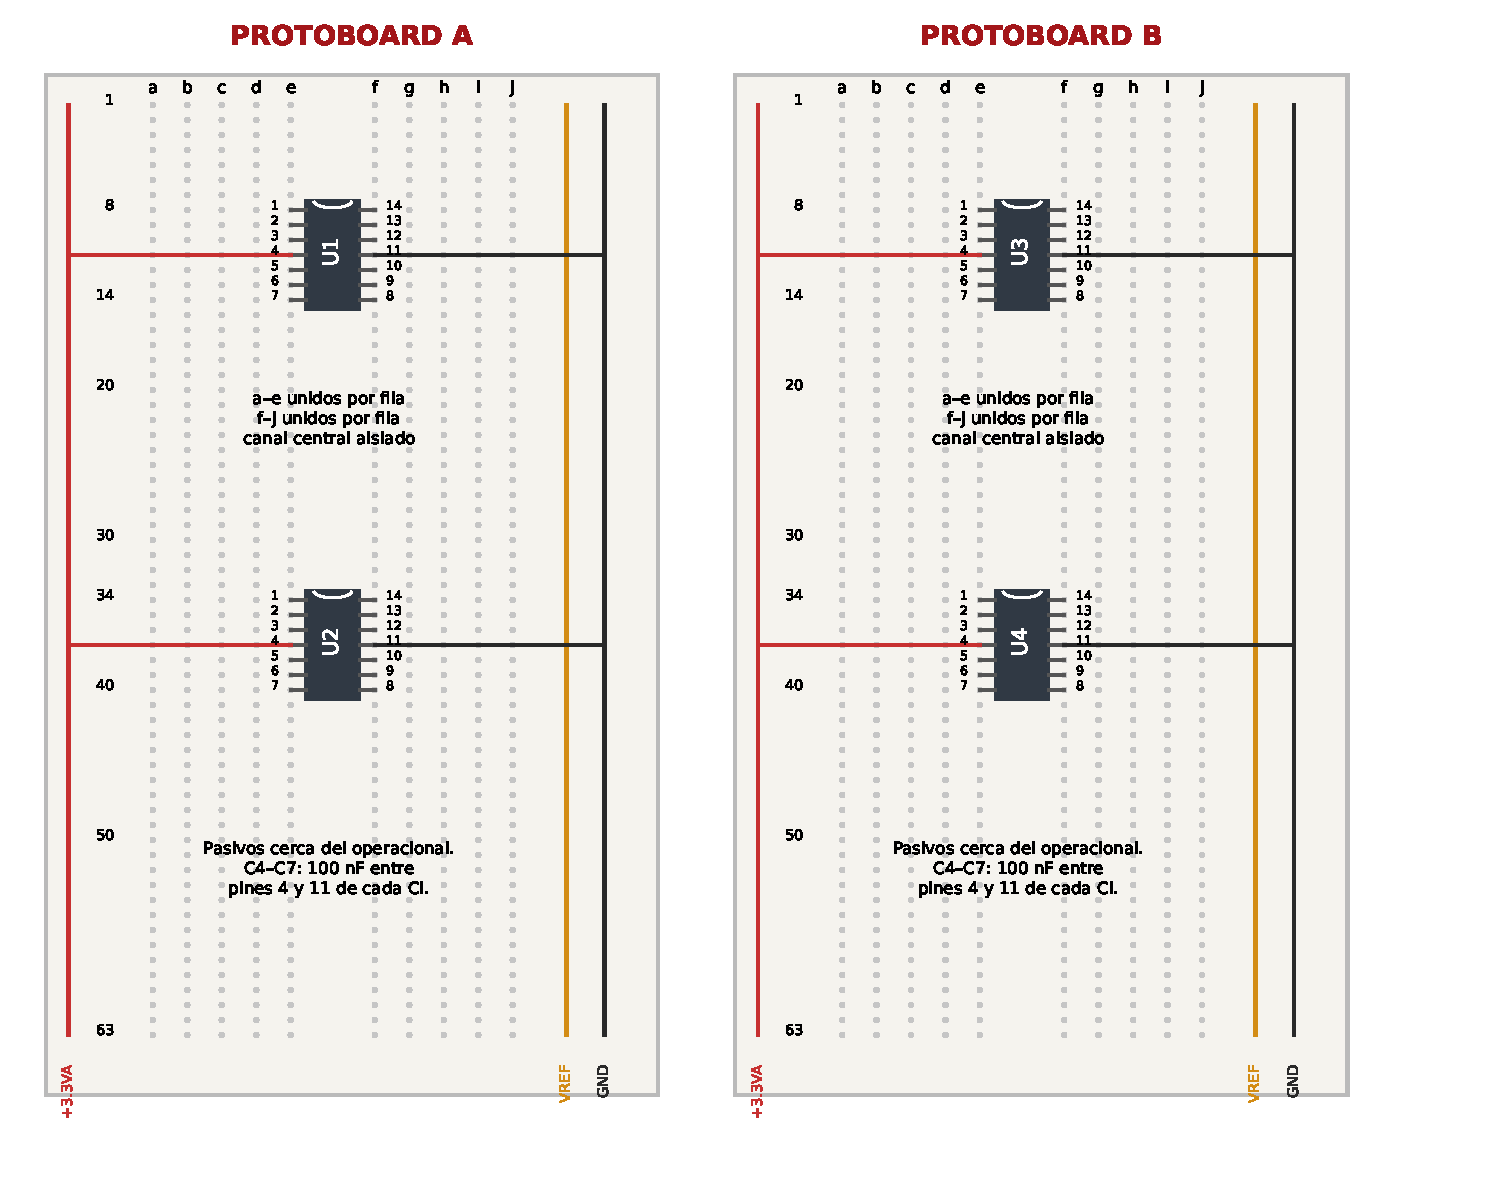
\includegraphics[width=.86\linewidth,height=176mm,keepaspectratio]{ubicacion-integrados.pdf}\end{center}
\textbf{Vista superior, muesca hacia arriba.} En cada integrado, el pin 1 queda arriba a la izquierda. Las filas de la placa A y la placa B se numeran por separado. Los pines atraviesan el canal central entre las columnas e y f. En una protoboard convencional, a--e están unidos dentro de la misma fila, y f--j forman otra unión independiente.

Este mapa fija la ubicación de U1--U4 y sus rieles; \textbf{no es un dibujo de todos los cables}. Las tablas posteriores indican cada conexión eléctrica. Distribuir los resistores y capacitores alrededor del operacional al que pertenecen, sin compartir una fila entre redes distintas. Los cruces de cables sobre el dibujo no significan unión.

\begin{tabularx}{\linewidth}{l X}\toprule
Placa / zona & Función\\\midrule
A, U1 en filas 8--14 & VREF, preamplificador, graves y primera etapa de medios.\\
A, U2 en filas 34--40 & Segunda etapa de medios, agudos, sumador y antialiasing.\\
B, U3 en filas 8--14 & Detectores y seguidores de graves y medios.\\
B, U4 en filas 34--40 & Detector de agudos, inversor de medios y unidad libre terminada en seguidor.\\\bottomrule
\end{tabularx}
Mantener cerca las placas A y B. El inversor de medios U4C se conecta al sumador U2C: no omitirlo aunque se deje el ESP32 desconectado.

\clearpage
\section{Esquema por etapas: entrada y filtros}
\etapa[65mm]{entrada}{Entrada estéreo mezclada a mono y preamplificador U1B.}
J1: T = canal izquierdo, R = canal derecho y S = GND. R4 y R5 evitan unir directamente las salidas izquierda y derecha. La ganancia de U1B en banda es aproximadamente $1+22/10=3,2$. El audio entra por C9; PRE tiene una componente continua próxima a VREF.
\etapa{graves}{Graves: filtro Sallen--Key pasa bajas, U1C.}
\clearpage
\subsection*{Filtros de medios y agudos}
\etapa{medios}{Medios: pasa altas U1D seguido de pasa bajas U2A; MED\_HP une ambas etapas.}
\etapa{agudos}{Agudos: filtro Sallen--Key pasa altas, U2B.}
Los valores nominales característicos son aproximadamente 232 Hz en graves, 409 Hz y 2,32 kHz en medios, y 4,09 kHz en agudos. Son frecuencias calculadas del diseño; comprobar la respuesta real con un barrido, sin confundirlas con medidas del prototipo.

\clearpage
\section{Controles, suma y señales para el ESP32}
\begin{figure}[H]\centering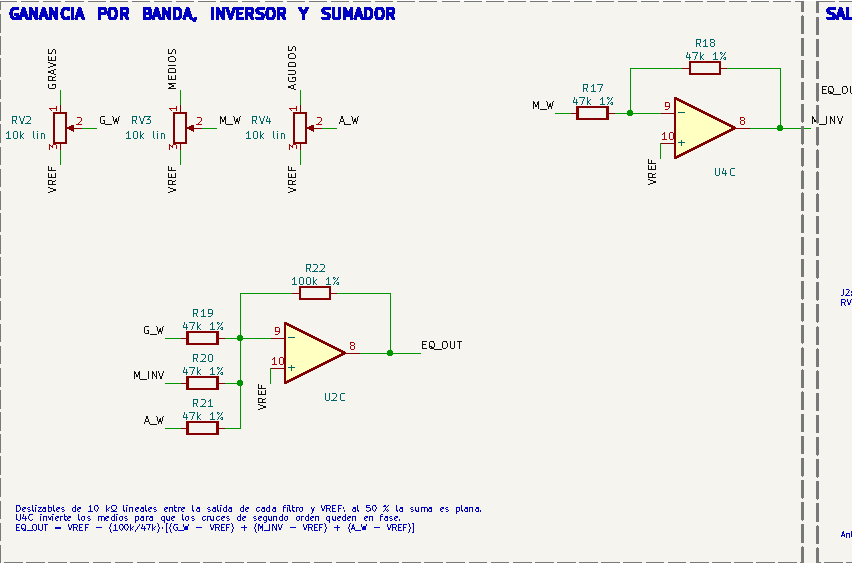
\includegraphics[width=.96\linewidth,height=85mm,keepaspectratio]{esquema-sumador.pdf}\caption{Ajuste por bandas, inversión de medios y sumador.}\end{figure}
En RV2--RV4, el extremo de señal recibe GRAVES, MEDIOS o AGUDOS; el otro extremo va a \textbf{VREF}, no a GND. Sus cursores son G\_W, M\_W y A\_W. El cursor de medios pasa por U4C antes del sumador. C19 elimina la continua de EQ\_OUT: su positivo va a EQ\_OUT y su negativo a OUT\_AC. Después de R23 se obtiene LINEA.

J2: T y R se conectan a LINEA; S a GND. Esta es una salida de línea para una entrada de alta impedancia, por ejemplo 10 k\ensuremath{\Omega} o más. No conectar directamente un parlante de 4 \ensuremath{\Omega} ni audífonos pasivos. El control RV5 y el PAM8403 corresponden solo a la opción de parlante interno.
\begin{figure}[H]\centering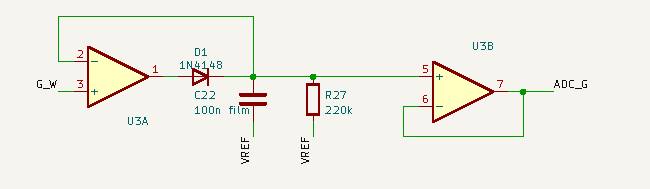
\includegraphics[width=.96\linewidth,height=48mm,keepaspectratio]{esquema-detector.pdf}\caption{Detector de graves. Medios y agudos repiten la estructura con sus propias referencias.}\end{figure}
En D1--D3, el ánodo va a DO\_G, DO\_M o DO\_A; el cátodo (extremo marcado con una banda) va a DET\_G, DET\_M o DET\_A. Los capacitores C22--C24 y resistencias R27--R29 retornan a VREF. Las salidas hacia el ESP32 son ADC\_G, ADC\_M y ADC\_A.
\begin{figure}[H]\centering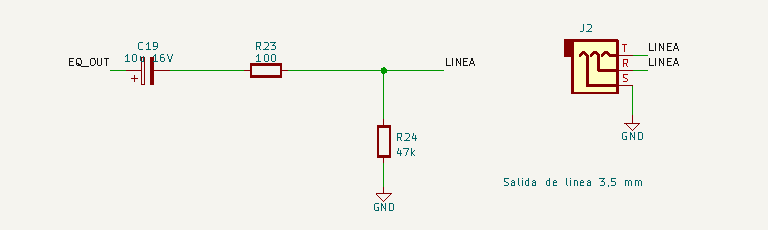
\includegraphics[width=.96\linewidth,height=55mm,keepaspectratio]{esquema-salida.pdf}\caption{C19, R23 y J2 forman la salida de línea. RV5 y J3 solo se usan con el PAM8403 opcional.}\end{figure}
\etapa{antialias}{U2D filtra EQ\_OUT antes de la entrada ADC\_FFT.}
Los detectores y el antialiasing pueden dejar sus salidas sin conectar durante las primeras pruebas; no es necesario instalar el ESP32 para comprobar el audio.

\clearpage
\section{Conexiones de los MCP6004, pin por pin}
Los nombres de red son los mismos del esquema. Si dos terminales tienen el mismo nombre, deben estar unidos eléctricamente, incluso si están en protoboards diferentes. La posición \red{A-e8} significa placa A, columna e, fila 8. No confundir el número de pin del integrado con el número de fila de la protoboard.

\begin{minipage}[t]{.48\linewidth}\subsection*{U1 · placa A}\begin{tabular}{r l p{39mm}}
\toprule Pin & Orificio & Red\\\midrule
1 & A-e8 & VREF\\
2 & A-e9 & VREF\\
3 & A-e10 & VDIV\\
4 & A-e11 & +3.3VA\\
5 & A-e12 & PRE\_IN\\
6 & A-e13 & PRE\_FB\\
7 & A-e14 & PRE\\
8 & A-f14 & GRAVES\\
9 & A-f13 & GRAVES\\
10 & A-f12 & LB2\\
11 & A-f11 & GND\\
12 & A-f10 & MH2\\
13 & A-f9 & MED\_HP\\
14 & A-f8 & MED\_HP\\
\bottomrule\end{tabular}
\end{minipage}\hfill
\begin{minipage}[t]{.48\linewidth}\subsection*{U2 · placa A}\begin{tabular}{r l p{39mm}}
\toprule Pin & Orificio & Red\\\midrule
1 & A-e34 & MEDIOS\\
2 & A-e35 & MEDIOS\\
3 & A-e36 & ML2\\
4 & A-e37 & +3.3VA\\
5 & A-e38 & AH2\\
6 & A-e39 & AGUDOS\\
7 & A-e40 & AGUDOS\\
8 & A-f40 & EQ\_OUT\\
9 & A-f39 & SUM\_N\\
10 & A-f38 & VREF\\
11 & A-f37 & GND\\
12 & A-f36 & AA2\\
13 & A-f35 & ADC\_FFT\\
14 & A-f34 & ADC\_FFT\\
\bottomrule\end{tabular}
\end{minipage}

\begin{minipage}[t]{.48\linewidth}\subsection*{U3 · placa B}\begin{tabular}{r l p{39mm}}
\toprule Pin & Orificio & Red\\\midrule
1 & B-e8 & DO\_G\\
2 & B-e9 & DET\_G\\
3 & B-e10 & G\_W\\
4 & B-e11 & +3.3VA\\
5 & B-e12 & DET\_G\\
6 & B-e13 & ADC\_G\\
7 & B-e14 & ADC\_G\\
8 & B-f14 & DO\_M\\
9 & B-f13 & DET\_M\\
10 & B-f12 & M\_W\\
11 & B-f11 & GND\\
12 & B-f10 & DET\_M\\
13 & B-f9 & ADC\_M\\
14 & B-f8 & ADC\_M\\
\bottomrule\end{tabular}
\end{minipage}\hfill
\begin{minipage}[t]{.48\linewidth}\subsection*{U4 · placa B}\begin{tabular}{r l p{39mm}}
\toprule Pin & Orificio & Red\\\midrule
1 & B-e34 & DO\_A\\
2 & B-e35 & DET\_A\\
3 & B-e36 & A\_W\\
4 & B-e37 & +3.3VA\\
5 & B-e38 & DET\_A\\
6 & B-e39 & ADC\_A\\
7 & B-e40 & ADC\_A\\
8 & B-f40 & M\_INV\\
9 & B-f39 & INV\_N\\
10 & B-f38 & VREF\\
11 & B-f37 & GND\\
12 & B-f36 & VREF\\
13 & B-f35 & U4D\_OUT\\
14 & B-f34 & U4D\_OUT\\
\bottomrule\end{tabular}
\end{minipage}

\textbf{U4D no se deja con las entradas flotantes:} conectar pin 12 a VREF y unir pines 13 y 14. Es el seguidor de reserva que ya aparece en el esquema.

\clearpage
\section{Conexiones de resistencias, capacitores y controles}
La tabla siguiente permite montar el circuito aunque no se disponga de KiCad. En un resistor o capacitor no polarizado, los extremos 1 y 2 son intercambiables. En C1, C8 y C19, el terminal 1 es el positivo. En los diodos, 1 es el cátodo y 2 el ánodo. En los potenciómetros, 2 es el cursor. C10 es bipolar en esta guía.
{\small\begin{longtable}{l p{44mm} p{96mm}}
\toprule Ref. & Valor & Terminal: red\\\midrule\endhead
R1 & 10 & 1: +3V3; 2: +3.3VA\\
C1 & 100u 10V & 1: +3.3VA; 2: GND\\
C2 & 100n & 1: +3.3VA; 2: GND\\
C4 & 100n & 1: +3.3VA; 2: GND\\
C5 & 100n & 1: +3.3VA; 2: GND\\
C6 & 100n & 1: +3.3VA; 2: GND\\
C7 & 100n & 1: +3.3VA; 2: GND\\
R2 & 10k 1\% & 1: +3.3VA; 2: VDIV\\
R3 & 10k 1\% & 1: VDIV; 2: GND\\
C8 & 10u 16V & 1: VDIV; 2: GND\\
R4 & 10k & 1: IN\_L; 2: MIX\\
R5 & 10k & 1: IN\_R; 2: MIX\\
RV1 & 10k log & 1: MIX; 2: NIVEL; 3: GND\\
C9 & 1u film & 1: NIVEL; 2: PRE\_IN\\
R6 & 100k & 1: PRE\_IN; 2: VREF\\
R7 & 22k 1\% & 1: PRE\_FB; 2: PRE\\
R8 & 10k 1\% & 1: PRE\_FB; 2: PRE\_G\\
C10 & 10 µF bipolar, \ensuremath{\geq} 10 V (ver nota C10) & 1: PRE\_G; 2: VREF\\
R9 & 10k 1\% & 1: PRE; 2: LB1\\
R10 & 10k 1\% & 1: LB1; 2: LB2\\
C11 & 100n film & 1: LB1; 2: GRAVES\\
C12 & 47n film & 1: LB2; 2: VREF\\
C13 & 10n film & 1: PRE; 2: MH1\\
C14 & 10n film & 1: MH1; 2: MH2\\
R11 & 27k 1\% & 1: MH1; 2: MED\_HP\\
R12 & 56k 1\% & 1: MH2; 2: VREF\\
R13 & 10k 1\% & 1: MED\_HP; 2: ML1\\
R14 & 10k 1\% & 1: ML1; 2: ML2\\
C15 & 10n film & 1: ML1; 2: MEDIOS\\
C16 & 4n7 film & 1: ML2; 2: VREF\\
C17 & 10n film & 1: PRE; 2: AH1\\
C18 & 10n film & 1: AH1; 2: AH2\\
R15 & 2k7 1\% & 1: AH1; 2: AGUDOS\\
R16 & 5k6 1\% & 1: AH2; 2: VREF\\
RV2 & 10 k\ensuremath{\Omega} lineal; rotativo o deslizable con cables & 1: GRAVES; 2: G\_W; 3: VREF\\
RV3 & 10 k\ensuremath{\Omega} lineal; rotativo o deslizable con cables & 1: MEDIOS; 2: M\_W; 3: VREF\\
RV4 & 10 k\ensuremath{\Omega} lineal; rotativo o deslizable con cables & 1: AGUDOS; 2: A\_W; 3: VREF\\
R17 & 47k 1\% & 1: M\_W; 2: INV\_N\\
R18 & 47k 1\% & 1: INV\_N; 2: M\_INV\\
R19 & 47k 1\% & 1: G\_W; 2: SUM\_N\\
R20 & 47k 1\% & 1: M\_INV; 2: SUM\_N\\
R21 & 47k 1\% & 1: A\_W; 2: SUM\_N\\
R22 & 100k 1\% & 1: SUM\_N; 2: EQ\_OUT\\
C19 & 10u 16V & 1: EQ\_OUT; 2: OUT\_AC\\
R23 & 100 & 1: OUT\_AC; 2: LINEA\\
R24 & 47k & 1: LINEA; 2: GND\\
R25 & 10k 1\% & 1: EQ\_OUT; 2: AA1\\
R26 & 10k 1\% & 1: AA1; 2: AA2\\
C20 & 4n7 film & 1: AA1; 2: ADC\_FFT\\
C21 & 2n2 film & 1: AA2; 2: VREF\\
D1 & 1N4148 & 1: DET\_G; 2: DO\_G\\
C22 & 100n film & 1: DET\_G; 2: VREF\\
R27 & 220k & 1: DET\_G; 2: VREF\\
D2 & 1N4148 & 1: DET\_M; 2: DO\_M\\
C23 & 100n film & 1: DET\_M; 2: VREF\\
R28 & 220k & 1: DET\_M; 2: VREF\\
D3 & 1N4148 & 1: DET\_A; 2: DO\_A\\
C24 & 100n film & 1: DET\_A; 2: VREF\\
R29 & 220k & 1: DET\_A; 2: VREF\\
\bottomrule\end{longtable}
}

\textbf{Conectores de audio:} en J1, T a IN\_L, R a IN\_R y S a GND; en J2, T y R a LINEA, S a GND. Si el jack incorpora contactos conmutados, identificar los terminales con un conector insertado y un multímetro: no usar el número de una pata del jack como si fuera universal.

\section{Ampliación con ESP32, pantalla y NeoPixel}
\subsection{Material adicional}
\begin{tabularx}{\linewidth}{r X}\toprule
Cant. & Material / referencias\\\midrule
1 & ESP32-DevKitC V4 de 38 pines, U5; adaptador de terminales o montaje externo con acceso a todos los pines.\\
1 & Waveshare 1,9 pulgadas, 170 × 320, ST7789V2; cable GH1.25 de 8 vías a 2,54 mm para J4.\\
1 & Pulsador SW1.\\
1 & 74AHCT125 en DIP-14, U6; no sustituir por 74HC125.\\
2 & Resistencias de 10 k\ensuremath{\Omega}: R30 y R32.\\
1 & Resistencia de 330 \ensuremath{\Omega}: R31.\\
1 de cada uno & C25 de 100 nF cerámico y C26 de 1000 µF, 10 V o más.\\
12 & LED WS2812B de una tira de 5 V; si se usan dos tramos, DOUT del primero a DIN del segundo.\\
1 & Fuente regulada de 5 V, 3 A, conexión J6; borneras para distribuir potencia fuera de la protoboard.\\
1 & Protoboard de 830 puntos adicional para U6 y conexiones auxiliares.\\\bottomrule
\end{tabularx}
No forzar el ESP32 sobre una protoboard si su ancho deja los terminales inaccesibles. Usar un adaptador o dos secciones separadas para alojar sus hileras. La pantalla se conecta por los nombres impresos de sus señales, no por una suposición sobre la orientación del conector.

\subsection{Entradas analógicas y pulsador}
\begin{tabularx}{\linewidth}{l l X}\toprule
Red & ESP32 & Origen / conexión\\\midrule
ADC\_G & GPIO34 & U3 pin 7: nivel de graves.\\
ADC\_M & GPIO35 & U3 pin 14: nivel de medios.\\
ADC\_A & GPIO32 & U4 pin 7: nivel de agudos.\\
ADC\_FFT & GPIO33 & U2 pin 14: salida del antialiasing.\\
VREF & GPIO36 / VP & U1 pines 1 y 2.\\
BTN & GPIO27 & SW1 entre GPIO27 y GND; pull-up interno en el firmware.\\
GND & GND & Retorno común con la parte analógica.\\\bottomrule
\end{tabularx}
Con el ESP32 todavía desconectado, verificar las tensiones de las cinco señales analógicas. Ninguna debe salir de 0 a 3,3 V. Para las pruebas iniciales del firmware, mantener las entradas medidas aproximadamente entre 0,15 y 2,45 V, el intervalo usado por la validación del proyecto. Si se alcanza ese límite o se aplana la señal, bajar RV1 antes de conectar el ADC.

\clearpage
\subsection{Pantalla Waveshare de 1,9 pulgadas}
\begin{tabularx}{\linewidth}{l l X}\toprule
Pantalla & Conexión & Observación\\\midrule
VCC & 3V3 & Riel digital de 3,3 V, antes de R1.\\
GND & GND & Retorno común.\\
DIN & GPIO23 & MOSI.\\
CLK & GPIO18 & Reloj SPI.\\
CS & GPIO5 & Selección de pantalla.\\
DC & GPIO21 & Datos/comandos.\\
RST & GPIO22 & Reinicio.\\
BL & GPIO19 & Control de luz; R30 de 10 k\ensuremath{\Omega} desde BL a GND.\\\bottomrule
\end{tabularx}
Conservar estos GPIO para usar el firmware del repositorio. Mantener cortos los cables de SPI. El firmware usa 40 MHz; si aparecen errores de imagen en protoboard, probar 10 MHz en \red{TFT_SPI_HZ}, definido en \red{firmware/include/config.h}, y recompilar el firmware. No cambiar los pines para resolver un problema de longitud de cable.

\subsection{Adaptador de nivel y tira LED}
\etapa{neopixel}{Datos NeoPixel: GPIO25, 74AHCT125 y resistencia de 330 \ensuremath{\Omega}.}
\begin{tabularx}{\linewidth}{l X}\toprule
Terminal & Conexión\\\midrule
U6 pin 14 & +5 V; C25 de 100 nF entre pin 14 y pin 7, cerca del integrado.\\
U6 pines 1 y 7 & GND. Pin 1 habilita la primera salida.\\
U6 pin 2 & GPIO25; R32 de 10 k\ensuremath{\Omega} desde esta unión a GND.\\
U6 pin 3 & R31 de 330 \ensuremath{\Omega}; el otro extremo de R31 a DIN de la tira.\\
U6 pines 4, 10 y 13 & +5 V: deshabilitan los tres canales no utilizados.\\
U6 pines 5, 9 y 12 & GND: fija las entradas no utilizadas.\\
U6 pines 6, 8 y 11 & Sin conexión. No unir estas salidas a GND.\\
Tira / C26 & +5 V y GND desde la distribución de potencia. C26: positivo a +5 V, negativo a GND.\\\bottomrule
\end{tabularx}
La corriente de la tira no debe atravesar el ESP32 ni las tiras de contactos de la protoboard: llevar +5 V y GND directamente desde la fuente a la tira mediante cables y borneras. Mantener la conexión de GND común con la lógica y la parte analógica. Empezar con brillo bajo y separar los cables LED de PRE\_IN, los filtros y SUM\_N.

\clearpage
\subsection{Cómo alimentar cada prueba}
\begin{enumerate}
\item \textbf{Solo analógico:} fuente regulada de 3,3 V a R1 y GND. No hace falta alimentar +5 V si no se instalan LED, ESP32 ni PAM8403.
\item \textbf{ESP32 y pantalla, sin cargas de potencia:} alimentar el DevKit por USB y usar su salida 3V3 para R1 y VCC de la pantalla. Retirar la fuente externa de 3,3 V; no unir dos reguladores al mismo riel.
\item \textbf{Montaje completo:} fuente externa de 5 V/3 A a la distribución J6. Desde allí: una rama al pin 5V del DevKit y otras ramas directas a LED y PAM8403, si se utiliza. La salida 3V3 del DevKit alimenta R1 y la pantalla. Mantener GND común, procurando que las corrientes de LED y parlante retornen a la fuente por sus propias ramas.
\end{enumerate}
Espressif indica que USB, entrada 5V y entrada 3V3 son formas de alimentación mutuamente excluyentes del DevKit. Para programar, desconectar la fuente externa de 5 V y usar USB. Si se requiere USB de datos durante la prueba con fuente externa, usar un adaptador que desconecte específicamente VBUS y conserve datos y GND, comprobado antes de conectar; un cable USB común no hace esa separación.

\subsection{Opción de parlante interno}
Agregar un módulo PAM8403, un parlante de 4 \ensuremath{\Omega}/3 W, RV5 de 10 k\ensuremath{\Omega} logarítmico y C3 de 470 µF/10 V. RV5: extremo 1 a LINEA, cursor a la entrada del canal elegido del módulo y extremo 3 a GND. Alimentar el módulo con +5 V y GND desde su rama de potencia; C3 entre esos dos terminales, con positivo a +5 V.

Conectar el parlante entre las salidas + y -- del \emph{mismo canal} del PAM8403. Ninguno de esos dos bornes es GND: no unir el negativo del parlante a la masa de la protoboard ni colocar allí la pinza de masa de un osciloscopio de banco. Para esta guía, medir la salida de línea J2, antes del amplificador de potencia. Los nombres y el orden de los terminales varían entre módulos: verificar la serigrafía del módulo adquirido.

\clearpage
\section{Orden de montaje y prueba}
\begin{enumerate}
\item \textbf{Sin alimentación:} identificar las uniones internas de las protoboards, puentear sus rieles si están divididos y colocar U1--U4 con la muesca hacia arriba. Revisar que +3.3VA, VREF y GND sean redes diferentes.
\item \textbf{Alimentación y referencia:} montar R1--R3, C1, C2, C4--C8 y U1A. Alimentar y medir +3.3VA, VDIV y VREF. Durante el montaje por etapas, mantener los operacionales aún no cableados en seguidor de VREF: entrada + a VREF, entrada -- unida a su salida. Retirar esos puentes temporales al construir cada etapa; no conectar su salida directamente a VREF.
\item \textbf{Entrada:} montar J1, R4--R8, RV1, C9 y C10. Poner RV1 inicialmente al mínimo. Para una señal mono de laboratorio, llevar la misma salida del generador a T y R de J1, antes de R4 y R5; no unir entre sí los canales de un celular.
\item \textbf{Filtros:} montar primero graves, luego las dos etapas de medios y después agudos. Comprobar cada salida antes de añadir el sumador.
\item \textbf{Suma:} instalar RV2--RV4, U4C y R17--R24, con C19 y J2. Comprobar que M\_W pasa por el inversor antes de llegar al sumador.
\item \textbf{Medición:} instalar antialiasing y detectores, incluidos D1--D3. Comprobar las tensiones en ADC\_G, ADC\_M, ADC\_A y ADC\_FFT antes de conectar el ESP32.
\item \textbf{Interfaz:} añadir ESP32 y pantalla; después, el adaptador de nivel y los LED. Agregar el PAM8403 solamente si se quiere probar la salida de parlante.
\end{enumerate}

\subsection{Prueba con generador y osciloscopio}
Configurar una senoide de \textbf{100 mVpp, sin offset}, medida en la entrada J1. Si el generador muestra amplitud para una carga de 50 \ensuremath{\Omega}, seleccionar modo Hi-Z o medir el valor real con el osciloscopio: la carga del circuito no es de 50 \ensuremath{\Omega}. Subir RV1 gradualmente hasta obtener aproximadamente 100 mVpp en PRE, sin recorte. Mantener los controles de banda en el mismo punto al comparar.

\begin{tabularx}{\linewidth}{l l X}\toprule
Frecuencia & Puntos de medida & Qué comprobar\\\midrule
100 Hz & PRE, GRAVES, MEDIOS, AGUDOS & Predominio de la salida de graves.\\
1 kHz & PRE, GRAVES, MEDIOS, AGUDOS & Predominio de la salida de medios.\\
8 kHz & PRE, GRAVES, MEDIOS, AGUDOS & Predominio de la salida de agudos.\\
Las tres anteriores & EQ\_OUT y LINEA & El control de la banda correspondiente cambia la amplitud. EQ\_OUT conserva polarización; LINEA queda centrada aproximadamente en 0 V.\\
Sin señal / con señal & ADC\_G, ADC\_M y ADC\_A & Reposo cerca de VREF; aumento de nivel con señal en su banda y descenso al retirarla.\\\bottomrule
\end{tabularx}
En las salidas internas, usar primero DC para verificar que la senoide esté centrada cerca de VREF, y luego AC para comparar amplitudes. Para un barrido, anotar $20\log_{10}(V_{salida}/V_{PRE})$ con el mismo tipo de medida en ambos canales: Vpp con Vpp, o RMS con RMS. No usar ADC\_FFT para evaluar la respuesta de agudos a 8 kHz: su filtro antialiasing introduce atenuación adicional.

\subsection{Si el montaje no funciona}
\begin{itemize}
\item VREF en 0 V: revisar R2/R3, alimentación de U1 y el puente entre pines 1 y 2; buscar una unión accidental de VREF con GND.
\item Salida pegada a un riel: verificar pinout, entradas +/--, continuidad de la realimentación y polarización antes de subir la amplitud.
\item Medios ausentes o respuesta distinta en los cruces: revisar U1D, U2A y el inversor U4C; no cambiar componentes antes de verificar el cableado.
\item Ruido al encender LED: probar sin tira para localizar el acoplamiento, revisar desacoples y retornos de potencia, y acortar cables de señal.
\item Imagen inestable: comprobar alimentación, nombres de los ocho cables de pantalla y longitud/frecuencia de SPI.
\end{itemize}

\section{Archivos y referencias}
El esquema vectorial completo se adjunta como última página de este PDF. Las tablas editables de compra y conexiones están en \red{docs/protoboard/materiales.csv} y \red{docs/protoboard/conexiones.csv}. El archivo fuente de esta guía es \red{docs/latex/prototipo-protoboard.tex}. El mapa de integrados no fija la ubicación de todos los pasivos; para éstos, seguir las conexiones pin--red de la tabla y del esquema.

\begin{itemize}
\item Microchip, \href{https://ww1.microchip.com/downloads/aemDocuments/documents/MSLD/ProductDocuments/DataSheets/MCP6001-1R-1U-2-4-1-MHz-Low-Power-Op-Amp-DS20001733L.pdf}{hoja de datos MCP6001/2/4}: encapsulado, terminales y alimentación del MCP6004.
\item Espressif, \href{https://docs.espressif.com/projects/esp-dev-kits/en/latest/esp32/esp32-devkitc/user_guide.html}{guía ESP32-DevKitC V4}: terminales y opciones de alimentación excluyentes.
\item Waveshare, \href{https://www.waveshare.com/wiki/1.9inch_LCD_Module}{1.9inch LCD Module}: interfaz y señales del módulo de 170 × 320.
\item Texas Instruments, \href{https://www.ti.com/lit/ds/symlink/sn74ahct125.pdf}{SN74AHCT125}: pinout y habilitación de los canales.
\end{itemize}

\clearpage
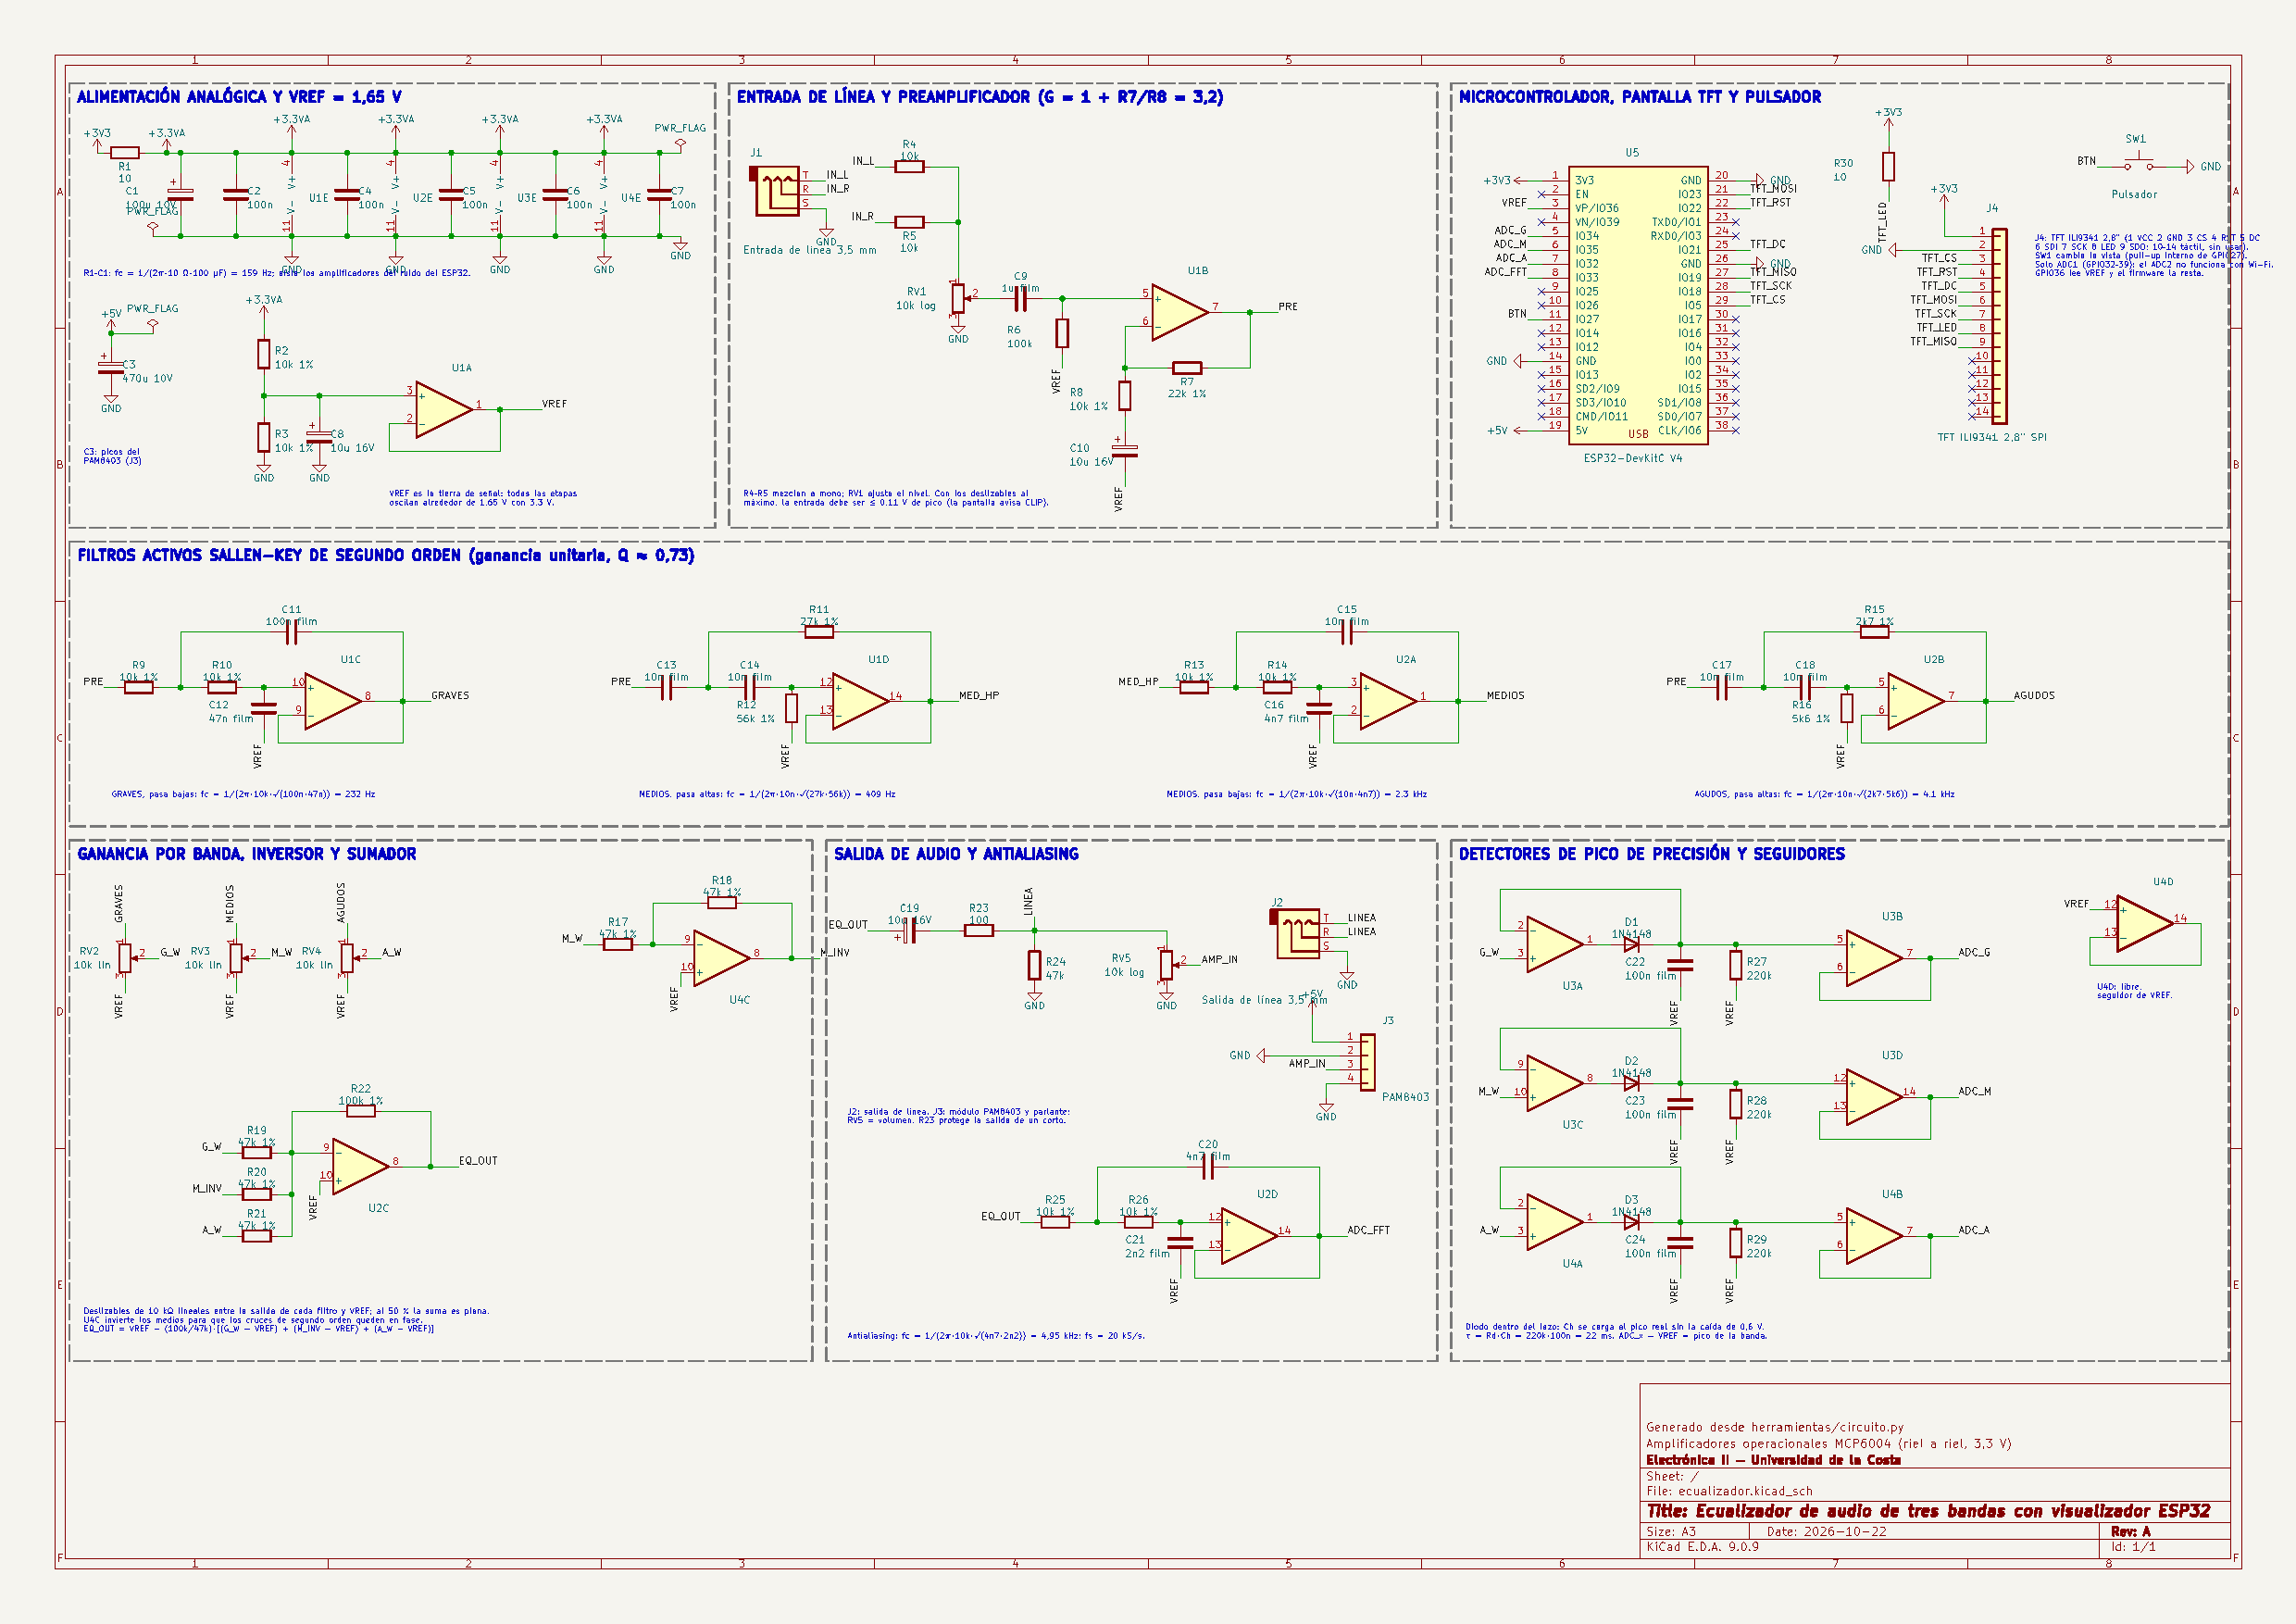
\includepdf[pages=-,fitpaper=true]{../../hardware/ecualizador.pdf}
\end{document}
